\chapter{Part 2}
\label{chap:Part2}
\section{Problem description}
The rating system is meant to be used as a movieguide. Relevant statistics help users choose movies they might find enjoyable. In order to choose a movie to watch, users can follow a number of different strategies ranging from simple to very sophisticated.

In the first part of this project, we considered algorithms for pairing up users with one friend. In the following, we will pair up users with multiple friends. By defining �types� of users, we can help users find other users with similar taste in movies. User �types� can also be helpful information for businesses in the processes of advertising and marketing.  

The users have rated the movies with a number from 1 to 5. We can build a graph where users having the same taste in movies are strongly connected, by computing weighted edges between the users, as in part 1.

\[weight = \frac{1}{n}\sum\limits_{i=1}^n 5 - | r^i_1 - r^i_2 |\]

where \(n\) is the number of movies rated by both users, and \(r_i^1\) and
\(r_i^2\) are the individual ratings given by the two users on the same movie,
denoted with the number i. 

We are looking for a solution where users are split into disconnected equally sized groups. Let T denote the sum of weights between the disconnected groups. Now, T is the value we are trying to minimize. Thus the partition we a looking for is not necessarily one where users with the same type have rated the same movies. As an example, consider the graph in figure \ref{fig:g1}.

\begin{figure}[h]
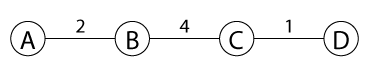
\includegraphics[width=300pt]{graph-cut.png}
\label{fig:g1}
\caption{}
\end{figure}

If we are to partition the graph into 2 equal sized sets, the intuitive solution might be to cut the graph in the middle, resulting in a T value of 4. While cutting the edges a-b and c-d instead, the value of T can be reduced 3.
Thus, with graphs such as this one, we will end up with a group of strongly connected users, and one of outsiders.
\section{Number of possible answers}
Lets consider the number of possible solutions to such a problem. We start by dividing n nodes into k subsets of size p. Picking the subsets one by one, our first pick is one out of (n p) possible first subsets. The second pick has ((n-p) * p) possible subsets, the third ((n-2*p) * p) possible subsets and so on. Since this must be done n/p = k times, and since the ordering of the subsets does not matter, the amount of possible solutions is:

\[ \frac{1}{k!}
    \left(\!\!\!\begin{array}{c}
      n \\
      p
    \end{array}\!\!\!\right) 
    \left(\!\!\!\begin{array}{c}
      n-p \\
      p
    \end{array}\!\!\!\right)
    ... 
    \left(\!\!\!\begin{array}{c}
      2p \\
      p
    \end{array}\!\!\!\right)
    \left(\!\!\!\begin{array}{c}
      p \\
      p
    \end{array}\!\!\!\right)
    \]
A number which becomes extremely large even for small sets of data. Finding a solution by looking at every possible answer to such a problem is impossible. Instead of finding the best possible solution, we will look at different strategies for finding good approximations.

\section{Different algorithms}
Practical solutions to graph partitioning problems are based on heuristics. The algorithms either use heuristics that rely on the properties of the graph as a whole, or rely on local searches. These are known as global and local heuristics.

Global heuristics typically uses analysis of the adjacency matrix to determine the partitions\cite{balanced}. Local strategies uses an arbitrary initial partition of the graph, which has major impact on the final outcome. A good property of the local algorithms is that they can be applied after a global algorithm, in order to improve the quality of the partition.

In this project we will implement an algorithm that uses local heuristics. 
\section{The Lin-Kernighan algorithm}
In order to find a k-way partitioning of a graph, we will start by solving a simpler problem: 2-way partitioning. When an algorithm for finding such a partitioning is found, we will extend it to solve the k-way partitioning problem.

The Lin-Kernighan algorithm improves an already partitioned graph. The quality of the final outcome is highly depended on the initial partition. The algorithm calculates how well-coupled each particular node is. If a node is connected strongly to other nodes with the same type, it is considered well-coupled. If it is connected to nodes of another type, it is loose-coupled. How loose a node is, is defined by

\[d=e-i\]

where e (external value) is the sum of weights of all edges going from the node to a node of a different partition, and i (internal value) is the sum of weight of all edges going from the node to nodes of the same partition. Furthermore, let T be the weight of all edges between subset A and B, the value we are trying to minimize.

Lemma 1 from \cite{linker} states that the reduction of T gained by swapping two nodes can be calculated by
\[reduction = a.d + b.d - 2 w(a,b)\]
where w(a,b) is the weight of the edges between node a and b if such edges exists.

Lin-Kernighan proceeds in the following way:

\begin{lstlisting}
First, determine d for all nodes.
Then repeat Q times:
        By lemma 1, find the nodes for with a swap will
        result in the highest possible gain.
        Swap those nodes and remove them from further
        considerations in this step.*
In the sequence of swaps executed, find what number of
swaps that results in the minimum T. Save only those
swaps and repeat the procedure. If no series of swaps
results in a lower T value, then terminate. 
\end{lstlisting}

* Note that the best possible swap does not necessarily result in a lower
T value. This mechanic makes it possible for the algorithm to perform a series
of swaps that overall results in a lower T value even though the individual
swaps does not.

Computing the d value for all nodes takes \(O(n^{2})\), since for every node, all other nodes must be considered. Finding the best possible swap with Lemma 1 takes \(O(n^{2})\) as well, and is very expensive because of the large amount of computations involved in each step. In our first na�ve implementation, the gain for every possible swap is computed. In the following section, we will describe how this procedure can be optimized.

The repeat value Q in the outer loop, is dependent of N, and so the computational complexity of the loop is \(O(n^{3})\). If the algorithm takes r passes, the computational complexity is \(O(rn^{2})\). Q is a value between 1 and \(|N|/2\). The higher Q is, the more swaps are considered in each step. The optimal value of Q depends on the graph. In the following section, we will try to determine the optimal value of Q. 

\section{Implementation}
We have implemented the Lin-Kernighan algorithm in ruby 2.0.0. LinKernighan.rb uses the graph implementation provided in Graph.rb, Edge.rb and Node.rb to find a graph partition. RatingsParser.rb parses the ratings and builds a graph. The implementation can be found in the lin-kernighan directory at the CD. The bin directory contains a shell script with a command line interface for feeding the algorithm input. Since the implementation is meant to be optimized for the MRI\cite{mri} version of Ruby, we have not used tail-recursion in our implementation.

\section{Evaluation}
In order to measure the quality of the solution found by our implementation, we compare the value of T before and after each run. Recall that T is the sum of external weights of the partitioned graph. The algorithm is executed with part of the MovieLens M1 dataset as input:

\begin{center}
\scalebox{0.9}{
\begin{tabular}{| l | l | l | l | l | l |}
\hline
Number of edges & Number of nodes & Q & CPU time/sec & T before & T after \\
\hline
10632 & 149 & 15 & 10.71 & 5709.60 & 5370.01       \\
35185 & 271 & 27 & 26.51 & 17961.94 & 17332.21     \\
79666 & 408 & 41 & 73.16 & 40284.27 & 38628.00     \\
136467 & 533 & 53 & 114.91 & 68392.38 & 66243.91   \\
215195 & 669 & 67 & 324.47 & 107504.96 & 103674.83\\
unknown & 6040 & 604 & unknown & unknown & unknown \\
\hline
\end{tabular}}
\end{center}

The seed to the random partition has been the same in every example. Only the time it takes the run the algorithm has been measured (Not the time used to parse the data). The time and T values are the average of 10 runs. A 2.4 Gz i5 core MacBook Pro was used as test machine. As the test data shows, the implementation is too slow to compute large dataset within a reasonable time. In order to improve execution speed, we used the profiler ruby-prof\cite{rubyprof} to find bottlenecks. We have introduced the following optimisations:
\begin{enumerate}
\item Nodes caches a list of their neighbours, and the edges leading to neighbours.
\item A hash of edges that can be looked up by node ids.
\item The d value of the nodes are recomputed lazily, and are only instructed to be lazily recomputed if neighbouring nodes have been swapped.
\end{enumerate}
However, after the optimizations the implementation was still too slow to compute large dataset within a reasonable time:

\begin{center}
\scalebox{0.9}{
\begin{tabular}{| l | l | l | l | l | l |}
\hline
Number of edges & Number of nodes & Q & CPU time/sec & T before & T after
\\
\hline
10632 & 149 & 15 & 5.20 & 5709.60 & 5370.01       \\
35185 & 271 & 27 & 15.58 & 17961.94 & 17332.21     \\
79666 & 408 & 41 & 53.56 & 40284.27 & 38628.00     \\
136467 & 533 & 53 & 90.73 & 68392.38 & 66243.91   \\
215195 & 669 & 67 & 243.39 & 107504.96 & 103674.83\\
unknown & 6040 & 604 & unknown & unknown & unknown \\
\hline
\end{tabular}}
\end{center}

The algorithm is highly dependent on the initial cut of the graph. To increase the chance of a cut with a low value of T, we can generate a number of random partitions, calculate the T value of each, and choose the partition with the lowest value. (In implementation, the seed to the random function resulting in best partition is used to recompute the graph.) Let Z denote the number of computed partitions. In order to estimate the best Z value of our test data, we run the following experiments:


Is seems that using the minimal T value of the random partition is not a good strategy. If anything, it leads a partition of lower quality. Let�s also consider the nature of the algorithm. By logging the reduction of T after each Q repeat, we can see that the biggest reduction of the T value lies at the first few steps:

\begin{center}
\begin{figure}[h]
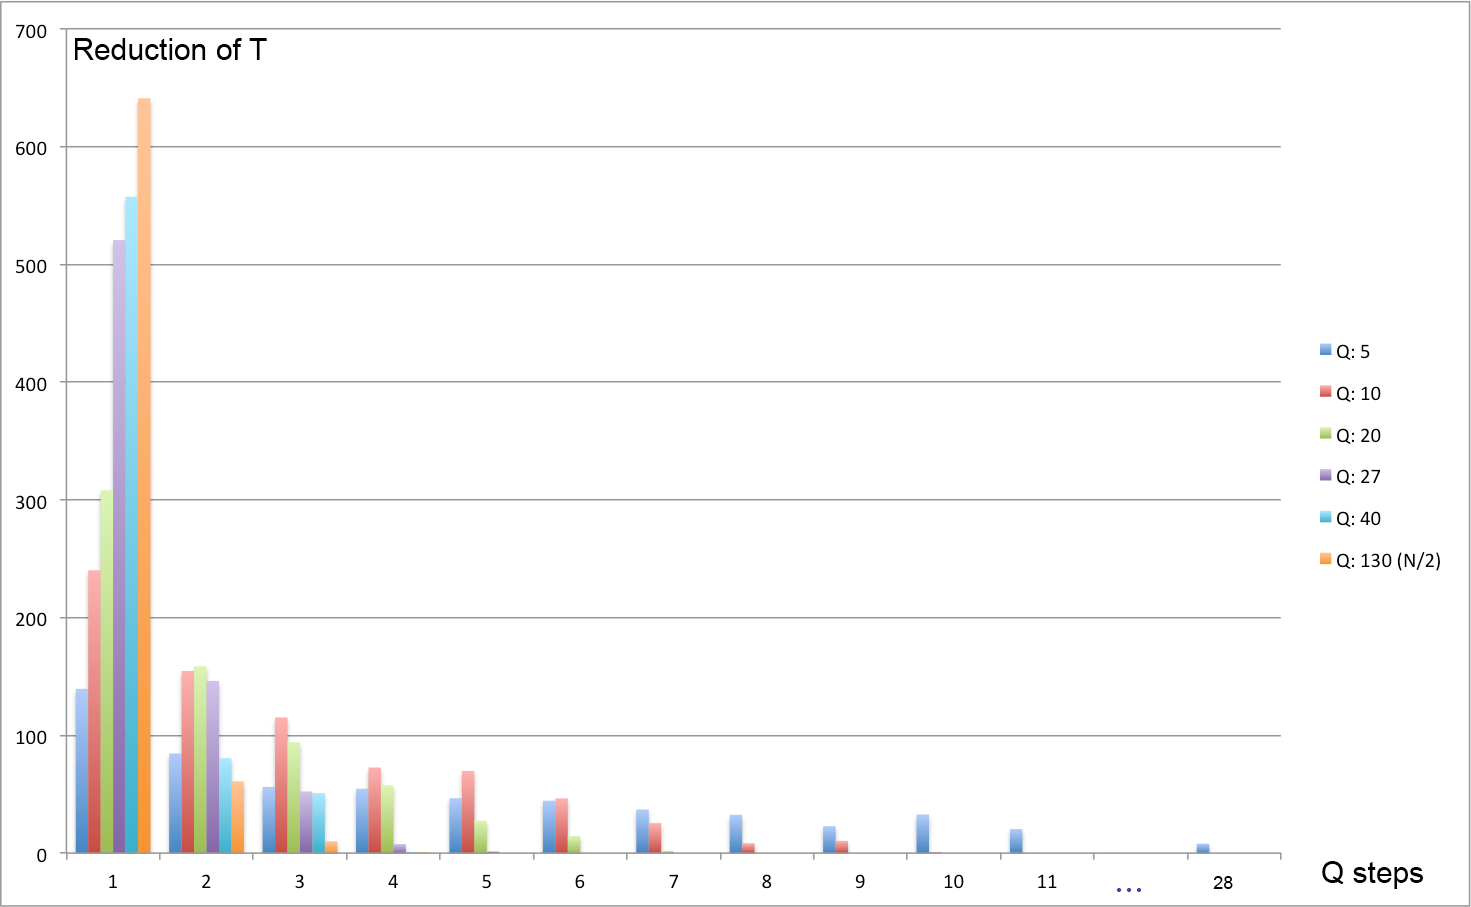
\includegraphics[width=300pt]{graph-cut3.png}

\label{fig:g3}
\end{figure}
\begin{figure}[h]
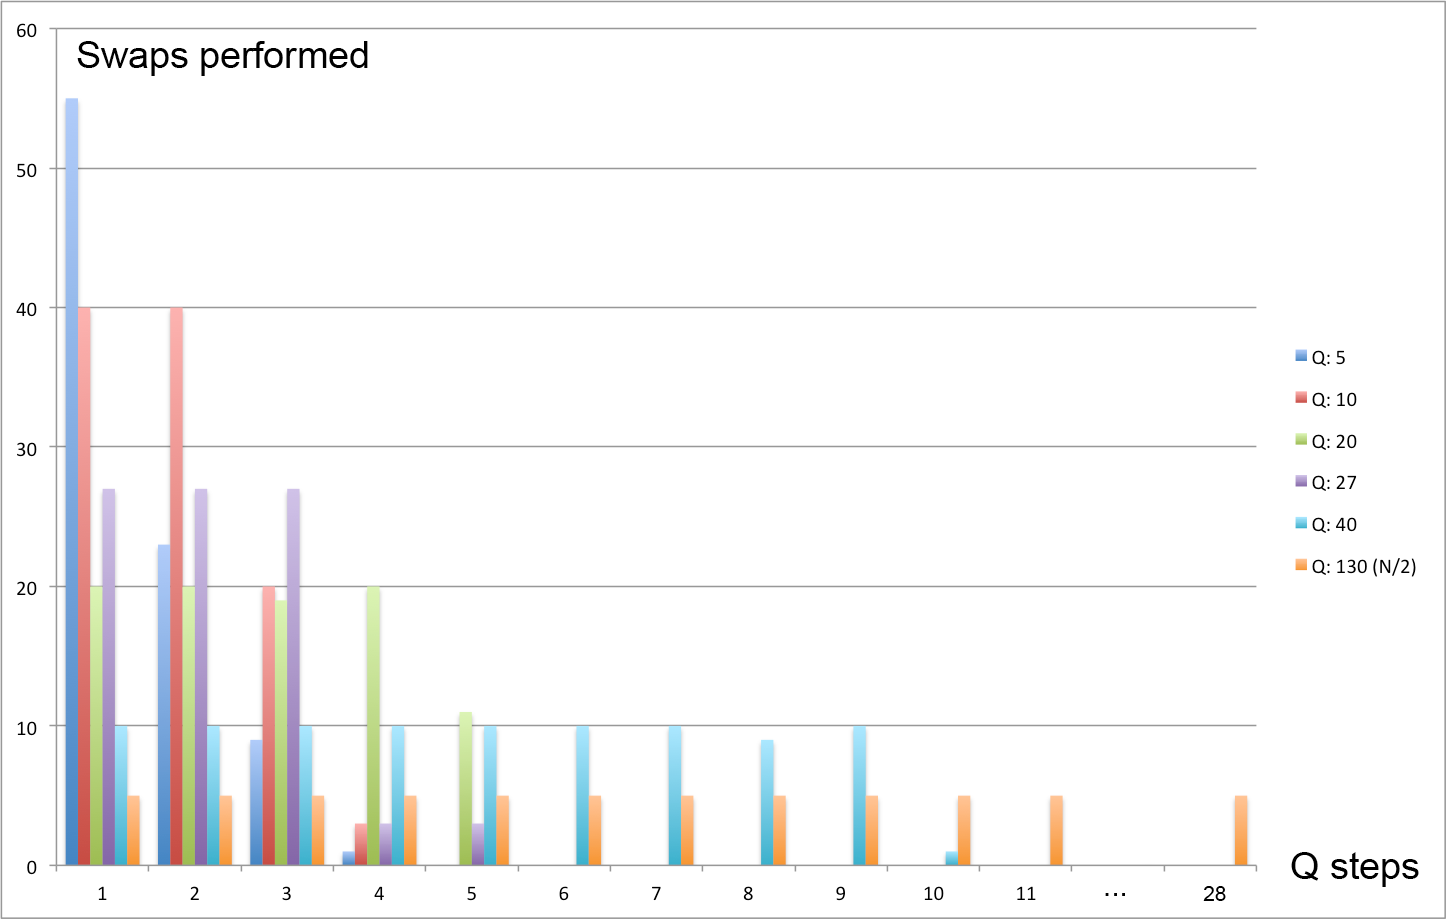
\includegraphics[width=300pt]{graph-cut4.png}
\label{fig:g4}
\end{figure}
\end{center}
As mentioned in the previous section, the task of computing the best possible swap is a \(O(n^2)\) procedure. It is currently the bottleneck of the computations. The gain from each swap is computed as shown in Lemma 1. Since no edges has negative weights, we know that \(-w(a,b)\) is 0 or negative. Therefore, the maximum gain possible by swapping two nodes is the sum of their d values. Let the nodes in each partition be sorted decreasingly by d, and lets compute the gain of each swap by going through the sorted nodes. If the maximum gain found is larger than the sum of d of the pair of nodes we are currently considering, then the computation can be stopped, since this pair and all the following pairs have a maximum possible gain lower than the maximum gain found. Notice, that we can no longer calculate the d values lazily, as the maximum d values must be found.

The computational complexity of finding the best possible swap is still \(O(n�2)\), but the reduction in runtime is significant:

\begin{center}
\scalebox{0.9}{
\begin{tabular}{| l | l | l | l | l | l |}
\hline
Number of edges & Number of nodes & Q & CPU time/sec & T before & T after
\\
\hline
10632 & 149 & 15 & 1.5 & 5659.73 & 5387.21       \\
35185 & 271 & 27 & 7.97 & 18035.91 & 17317.79     \\
79666 & 408 & 41 & 36.95 & 40250.41  & 38840.32     \\
136467 & 533 & 53 & 98.10 & 68345.01 & 66127.00   \\
215195 & 669 & 67 & 141.68 & 107387.44  & 103839.21\\
unknown & 6040 & 604 & unknown & unknown & unknown \\
\hline
\end{tabular}}
\end{center}

Notice that the algorithm only needs to calculate the gain from about 2-3 nodes from each array. The computational complexity of calculating the best swap is now in practice bound by the sorting.

Even after the optimizations, the implementation cannot compute the data within a reasonable amount of time. We shall return to a discussion of this problem, for now, lets consider our options for producing a k-way partition:

\section{From a 2-way partition to a k-way partition}
To make the algorithm find multiple partitions, we apply it multiple times. The graph is split into two partitions of equal size, and then recursively applied to each partition. In order to improve the quality of the solutions found by this approach, we can implement an extra step. After the first two splits, the partitions found by the second split are combined, and then split again. If the T value of this third split is better than the previous one, then it is chosen. The strategy is illustrated in the following figure:

\begin{figure}[h]
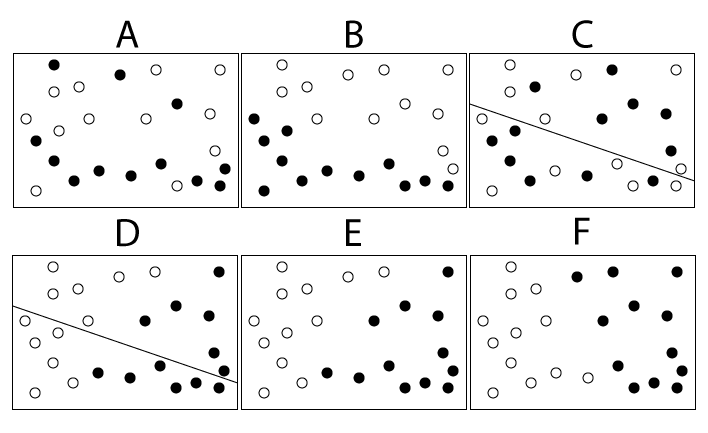
\includegraphics[width=300pt]{graph-cut2.png}
\label{fig:g2}
\end{figure}

A) A random partition is found, B) The algorithm is run. C) Random partitions are found on each partition. D) The algorithm is run on each partition. E) The partitions are merged. F) The algorithm is run (without a random partition). Now, the T value is calculated for the result in B and F. The result with the lowest T value is chosen as the partition. This strategy will improve the outcome of the algorithm, but increase the run time.

\section{Retrospect}

During the implementation of the Lin-Kernighan algorithm, we have realized a number of things that we would have liked to do differently. The Lin-Kernighan algorithm is not efficient enough to process such a big dataset. The strength of the algorithm is not the first partition of the graph. Rather, since the algorithm works on already partitioned graphs, it should be used to improve the solutions found by other algorithms. See \cite{schulz} for an example. The Lin-Kernighan algorithm works as  a basecase for other local heuristic
methods. In \cite{dutt}, it is shown the that the time complexity can be
reduced to  \(O(max(d|E|, |E| log |N|))  \)\footnote{d is the maximum number of outgoing edges from any node}, by only swapping neighboring nodes.
In order process such a large amount of data, algorithms depending on global heuristics would be a better choice.\cite{naor} 

The Ruby language is not very suitable for algorithms requiring large amounts of computations. It is difficult to reason about the time complexity of the methods of the datastructures in the standard library. A better choice would have been a language such as C or C++.
\section{Conclusion}
Throughout the project we have studied a range of algorithmic problems related to movie ratings in the MovieLens dataset. In the first part of the report we have covered different techniques for calculating average ratings. While not algorithmic difficult, this allowed us to discuss different approaches of streaming and MapReduce with a simple example. Next we considered ways to find movie buddies by applying algorithms for finding approximate maximum weighted matchings in a dense graph. First a �-approximation sequential approach, which was implemented, and then we discussed an 8-approximation MapReduce approach for graphs too big to fit in memory on a single machine exploiting a technique called filtering. 

In the second part of the project, we have introduced the field of graph partitioning. We have seen how simple data such as the user ratings can yield complex algorithmic problems. We have implemented a heuristic graph algorithm, and discussed its inner workings. We have seen how statistical information can help optimize an algorithm for a particular dataset. We have also seen how a dataset can be so big that even an optimised algorithm is not efficient enough to process it. Finally, we have discussed  why a different type of algorithm might have been a more suitable choice.



 





